\section{Implementación del software}

En esta sección voy a describir cómo llevamos a la práctica el Sistema de Carnetización Digital y Gestión de Eventos, ese proceso de aterrizar todas las ideas del diseño en un producto funcional que realmente se pudiera usar. Aquí es donde la teoría se encuentra con la realidad del código, donde los diagramas se convierten en líneas de programación y donde las decisiones arquitectónicas empiezan a mostrar sus consecuencias —para bien o para mal—. Voy a explicar la arquitectura que elegimos, las principales decisiones tecnológicas que tuvimos que tomar (y por qué las tomamos así), y la forma en que organizamos todo el trabajo de desarrollo, incluyendo pruebas, automatización y despliegue.

El objetivo de esta sección no es solo mostrar qué construimos, que al final del día es "otra app más". Lo que realmente quiero que se entienda es por qué tomamos cada decisión técnica específica, cómo estas elecciones se conectan directamente con una realidad que manejan muchas empresas que necesitan un control de asistencia, y cómo se ajustan al alcance de un proyecto académico que tiene limitaciones reales de tiempo, presupuesto y experiencia del equipo, pero que aspira a generar un impacto medible y duradero.

\subsection{Arquitectura del sistema}

La arquitectura que adoptamos se diseñó pensando en tres necesidades muy concretas que identificamos desde el principio: que el sistema fuera realmente fácil de mantener a largo plazo, que pudiera crecer y evolucionar en el futuro sin necesidad de reescribirlo desde cero, y —esto es crucial— que cualquier aprendiz del programa ADSO que llegue después pudiera entenderlo y continuarlo sin tener que descifrar un código misterioso o una estructura caótica. No queríamos crear un proyecto que funcionara solo mientras nosotros estuviéramos ahí para sostenerlo.

Por esta razón optamos por una estructura por capas bien definida, separando claramente el frontend (las interfaces que ve y con las que interactúa el usuario), el backend (donde vive toda la lógica de negocio y la API que orquesta todo), y la base de datos (donde se almacena persistentemente toda la información crítica del sistema). Esta separación no es solo un capricho académico o una moda arquitectónica; tiene consecuencias prácticas muy concretas: si mañana necesitamos cambiar la interfaz web por una completamente diferente, podemos hacerlo sin tocar una sola línea del backend. Si más adelante queremos migrar la base de datos a otro motor, el impacto en el resto del sistema será mínimo porque todo pasa por una capa de abstracción bien diseñada.

En la capa web utilizamos Angular para construir la plataforma administrativa, ese panel de control donde los coordinadores académicos pueden gestionar aprendices, crear y configurar eventos, consultar en tiempo real quién ha llegado, y generar los reportes que necesitan para sus procesos administrativos. Angular nos dio una estructura opinada muy clara sobre cómo organizar componentes, servicios y rutas, lo cual fue invaluable para mantener el código ordenado cuando el proyecto empezó a crecer más allá de las primeras pantallas prototipo.

En la capa móvil elegimos React Native para ofrecer una aplicación ligera, rápida y multiplataforma que funciona tanto en Android como en iOS sin tener que mantener dos bases de código completamente separadas. Esta app está enfocada casi exclusivamente en una experiencia de usuario súper fluida para el escaneo de códigos QR: abres la aplicación, apuntas con la cámara al código del carné o del evento, y en cuestión de segundos recibes una confirmación visual y sonora de que tu asistencia quedó registrada correctamente en el sistema. Nada de formularios complicados, nada de menús confusos, solo la funcionalidad esencial presentada de la manera más directa posible.

El backend se construyó con .NET y C\#, exponiendo una API REST bien documentada que centraliza absolutamente toda la lógica relacionada con usuarios, roles y permisos, generación de carnés digitales con códigos QR únicos, registro de asistencias a eventos, y toda la orquestación de datos que hace funcionar el sistema. Esta API se conecta a una base de datos PostgreSQL, que elegimos muy conscientemente por su estabilidad probada en producción, su excelente soporte para relaciones complejas entre tablas (algo fundamental cuando tienes entidades como usuarios, eventos, asistencias, roles, permisos, etc., todas interrelacionadas), y su compatibilidad demostrada con los servicios y la infraestructura que actualmente manejan multiples organizaciones como por ejemplo el SENA.

Desde el punto de vista operativo, tengo que ser honesto: aunque el proyecto no cuenta con un entorno corporativo completo de DevOps con servidores dedicados, pipelines sofisticados de CI/CD y toda la infraestructura que tendrías en una empresa grande, sí adoptamos conscientemente prácticas inspiradas directamente en esos lineamientos profesionales. Implementamos control de versiones riguroso con Git usando ramas de trabajo bien definidas (development, staging, main), integración de pruebas automatizadas básicas que se ejecutan antes de cada merge, y scripts de despliegue reproducibles y documentados que reducen dramáticamente los errores humanos al mover el sistema entre el ambiente de desarrollo local y el servidor de producción. La idea fue acercarnos lo más posible a estándares profesionales dentro de nuestras limitaciones reales.

A nivel de experiencia de usuario, la arquitectura completa se pensó meticulosamente para que el flujo de interacción fuera lo más simple, intuitivo y rápido posible. El aprendiz solo necesita realizar tres acciones básicas: abrir la app móvil en su teléfono, apuntar la cámara al código QR de su carné digital o al código del evento al que quiere asistir, y recibir una confirmación inmediata —visual con un ícono de éxito y sonora con un pequeño tono— de que su registro quedó guardado correctamente en el sistema. Todo esto en menos de cinco segundos.

Mientras tanto, del otro lado, el instructor o el administrador puede ver en la plataforma web, prácticamente en tiempo real gracias a las actualizaciones automáticas, quién ha ingresado al evento, cuántos cupos se han ocupado ya, si alguien está faltando sistemáticamente a las sesiones, y puede exportar reportes detallados en formato Excel o PDF cuando lo requiera para sus procesos administrativos o para enviar a coordinación académica. Este enfoque de diseño centrado en el usuario responde directamente a los problemas concretos que identificamos tanto en nuestra experiencia personal como en la literatura científica: reducir drásticamente los tiempos de espera que se generaban con el método manual, evitar las filas innecesarias que se formaban en las puertas, eliminar los errores de transcripción que plagaban las listas físicas, y sobre todo, transformar la asistencia de ser un simple dato archivado en un papel que nadie vuelve a consultar, en información confiable, actualizada y disponible inmediatamente para la gestión educativa y la toma de decisiones estratégicas.

\subsection{Prácticas de desarrollo y calidad}

Aunque se trata fundamentalmente de un proyecto académico desarrollado en el contexto de nuestra formación como tecnólogos, hicimos un esfuerzo muy consciente y deliberado por trabajar con hábitos y prácticas lo más cercanos posible a los de un equipo profesional de desarrollo de software en una empresa real. No queríamos que el proyecto fuera "solo otro entregable de clase" que se hace a las carreras, se entrega para cumplir con la nota y luego se abandona para siempre. Queríamos construir algo que realmente pudiera evolucionar y mantenerse en el tiempo.

Desde el primer día de desarrollo definimos convenciones claras de formateo y estilo de código para todos los lenguajes que estábamos usando. Configuramos herramientas automáticas de \textit{linting} (análisis estático de código) para C\# en el backend, TypeScript en el frontend web de Angular, y JavaScript en la aplicación móvil de React Native. Estas herramientas revisan automáticamente el código en busca de problemas comunes de estilo, inconsistencias de formato, posibles errores lógicos y malas prácticas conocidas. El objetivo era mantener un estilo consistente y profesional en toda la base de código, lo que facilita enormemente que otros compañeros del equipo —o futuros aprendices que hereden el proyecto— puedan leer, entender y modificar el código sin perder tiempo tratando de descifrar "manías" personales de formateo o estructuras extrañas que solo tienen sentido para quien las escribió originalmente.

En el backend implementamos pruebas unitarias automatizadas para todas las partes críticas de la lógica de negocio, esas funciones que si fallan pueden comprometer todo el sistema. Específicamente, escribimos pruebas exhaustivas para el registro de asistencia (¿qué pasa si el QR es inválido? ¿qué pasa si el evento ya terminó? ¿qué pasa si alguien intenta registrarse dos veces?), la validación de credenciales de usuario (¿se están hasheando correctamente las contraseñas? ¿se rechazan intentos de login con credenciales incorrectas?), y la generación de códigos QR únicos (¿se están generando códigos realmente únicos? ¿se están asociando correctamente con cada usuario?). Estas pruebas automatizadas se ejecutan cada vez que alguien hace un commit importante, dándonos confianza de que no estamos "rompiendo" funcionalidad que ya funcionaba.

Para los componentes de frontend, donde las pruebas automatizadas de interfaz gráfica son más complejas de implementar y mantener, realizamos pruebas manuales exhaustivas pero guiadas sistemáticamente por casos de uso reales que documentamos en detalle: creación de un evento desde cero con todos sus parámetros, escaneo exitoso de carnés en diferentes condiciones de iluminación, recuperación de contraseña olvidada siguiendo todo el flujo de emails, generación de reportes con diferentes filtros y formatos de exportación, manejo de errores cuando no hay conexión a internet, etc. Cada caso de uso tiene una lista de verificación paso a paso que seguimos religiosamente antes de dar por terminada una funcionalidad.

Además, incorporamos un análisis estático de seguridad sencillo pero efectivo que se ejecuta automáticamente antes de cada despliegue a producción. Este análisis revisa advertencias comunes y peligrosas como posibles inyecciones de SQL (cuando se construyen consultas concatenando strings sin sanitizar), control insuficiente de errores que podría dejar el sistema en un estado inconsistente, exposición accidental de información sensible en logs o mensajes de error, y uso de librerías con vulnerabilidades de seguridad conocidas. No es un análisis exhaustivo de nivel corporativo, pero sí nos ayuda a evitar los errores de seguridad más comunes y tontos.

El flujo de entrega del proyecto se organizó en pequeños \textit{sprints} de dos semanas siguiendo la metodología Scrum que habíamos seleccionado en nuestra comparación de metodologías ágiles. Al final de cada iteración construíamos una versión funcional y desplegable del sistema completo, la probábamos  con datos de prueba realistas que simulaban escenarios reales de organizaciones, y documentábamos cuidadosamente todos los cambios relevantes tanto en el código como en la funcionalidad visible para el usuario. Esta documentación no era solo para nosotros; era pensando en que cualquier instructor, coordinador o futuro desarrollador pudiera entender qué hace cada versión y qué cambió respecto a la anterior.

Aunque no disponemos de una cadena completa de \textit{continuous delivery} con servidores dedicados de staging y producción, balanceadores de carga, monitoreo 24/7 y todo lo que tendría una infraestructura corporativa madura, sí simulamos conscientemente este enfoque profesional mediante scripts que desarrollamos nosotros mismos y que automatizan todo lo automatizable: el empaquetado del backend en un contenedor Docker, la ejecución de migraciones de base de datos para actualizar el esquema sin perder datos, la construcción optimizada de las aplicaciones cliente web y móvil, y el despliegue coordinado de todos estos componentes. Estos scripts reducen dramáticamente el riesgo de "romper" el sistema al hacer ajustes de última hora o al mover código entre ambientes, porque eliminan los pasos manuales donde típicamente se cometen errores humanos.

\subsection{Fragmento representativo de código}

En lugar de mostrar una función genérica y abstracta que no dice mucho sobre lo que realmente hace el sistema, decidí presentar un fragmento de código que refleja directamente la lógica central del proyecto, la razón de ser de toda esta arquitectura: el registro de la asistencia de un aprendiz a un evento a partir del escaneo de su código QR personal. Este ejemplo ilustra varias decisiones de diseño importantes: el uso de tipado estático fuerte en C\# que previene muchos errores en tiempo de compilación, la validación cuidadosa de cada paso antes de guardar cualquier cosa en la base de datos para mantener la integridad de los datos, y el manejo explícito de todos los casos de error posibles para dar feedback claro al usuario.

\ifminted
\begin{minted}[linenos, fontsize=\small]{csharp}
public async Task<AttendanceResult> RegisterAttendanceAsync(
    Guid eventId,
    string qrValue,
    string deviceId)
{
    // 1. Buscar el aprendiz asociado al QR escaneado
    var person = await _personData.FindByQrAsync(qrValue);
    if (person is null)
    {
        return AttendanceResult.Failed(
            "Carné no válido o no registrado en el sistema.");
    }

    // 2. Verificar que el evento exista y esté activo
    var @event = await _eventData.GetActiveByIdAsync(eventId);
    if (@event is null)
    {
        return AttendanceResult.Failed(
            "El evento no está disponible o ya finalizó.");
    }

    // 3. Verificar que no haya un registro duplicado
    var exists = await _attendanceData.ExistsAsync(eventId, person.Id);
    if (exists)
    {
        return AttendanceResult.Failed(
            "Ya registraste tu asistencia a este evento.");
    }

    // 4. Registrar la asistencia con timestamp preciso
    var attendance = new Attendance
    {
        EventId = eventId,
        PersonId = person.Id,
        DeviceId = deviceId,
        RegisteredAt = DateTime.UtcNow
    };

    await _attendanceData.AddAsync(attendance);
    return AttendanceResult.Success(person.FullName, @event.Name);
}
\end{minted}
\else
\begin{lstlisting}[language={[Sharp]C},numbers=left, basicstyle=\small\ttfamily]
public async Task<AttendanceResult> RegisterAttendanceAsync(
    Guid eventId,
    string qrValue,
    string deviceId)
{
    // 1. Buscar el aprendiz asociado al QR escaneado
    var person = await _personRepository.FindByQrAsync(qrValue);
    if (person is null)
    {
        return AttendanceResult.Failed(
            "Carné no válido o no registrado en el sistema.");
    }

    // 2. Verificar que el evento exista y esté activo
    var @event = await _eventData.GetActiveByIdAsync(eventId);
    if (@event is null)
    {
        return AttendanceResult.Failed(
            "El evento no está disponible o ya finalizó.");
    }

    // 3. Verificar que no haya un registro duplicado
    var exists = await _attendanceData.ExistsAsync(eventId, person.Id);
    if (exists)
    {
        return AttendanceResult.Failed(
            "Ya registraste tu asistencia a este evento.");
    }

    // 4. Registrar la asistencia con timestamp preciso
    var attendance = new Attendance
    {
        EventId = eventId,
        personId = person.Id,
        DeviceId = deviceId,
        RegisteredAt = DateTime.UtcNow
    };

    await _attendanceRepository.AddAsync(attendance);
    return AttendanceResult.Success(person.FullName, @event.Name);
}
\end{lstlisting}
\fi

Este fragmento de código resume varias decisiones arquitectónicas fundamentales que tomamos desde el inicio: mantener toda la lógica de negocio correctamente encapsulada en servicios reutilizables que pueden ser llamados desde cualquier controlador o endpoint de la API, trabajar con el patrón de repositorio para aislar completamente el acceso a datos y hacer que sea fácil cambiar la implementación de persistencia sin afectar la lógica de negocio, y devolver resultados explícitos y bien tipados al frontend que luego se traducen automáticamente en mensajes comprensibles para el usuario final: "asistencia registrada exitosamente", "evento no disponible", "carné no válido", "ya registraste tu asistencia", etc. Este diseño hace que el sistema sea predecible, testeable y fácil de mantener.

\subsection{Comparación y justificación de tecnologías}

La elección final de Angular para web, React Native para móvil, .NET para backend y PostgreSQL para base de datos no fue para nada casual ni basada únicamente en preferencias personales o en "lo que ya conocíamos". Durante toda la fase inicial de diseño del proyecto dedicamos tiempo significativo a comparar sistemáticamente diferentes alternativas de frameworks web y móviles, considerando cuidadosamente criterios objetivos como: la curva de aprendizaje realista para nuestro equipo que tenía experiencia limitada con algunas de estas tecnologías, la existencia de una comunidad activa y documentación abundante en español que pudiéramos consultar cuando nos atascáramos (que inevitablemente iba a pasar), la facilidad de integración con APIs REST que es el estándar de facto para comunicación entre frontend y backend, y las posibilidades reales de despliegue en la infraestructura que actualmente maneja el SENA sin requerir servidores especializados o configuraciones exóticas.

En el caso específico de los frameworks frontend evaluamos en detalle opciones como Angular (el que finalmente elegimos), React puro sin framework adicional, y Vue.js que también es muy popular. Para el backend analizamos exhaustivamente .NET Core (nuestra elección final), Node.js con Express que es muy usado en startups, Spring Boot de Java que es el estándar corporativo en muchas empresas grandes, y algunos frameworks de PHP como Laravel que tiene mucha presencia en desarrollo web tradicional. Para la base de datos comparamos principalmente PostgreSQL (que elegimos) y MySQL que es probablemente más conocido, pero también consideramos brevemente opciones NoSQL como MongoDB para entender si realmente necesitábamos una base relacional o no.

La Tabla \ref{tab:frameworks} resume de manera condensada esta comparación multi-criterio, resaltando que Angular ofrece una estructura muy clara y opinada sobre cómo organizar un proyecto mediano, algo extremadamente valioso para un equipo en formación que puede perderse fácilmente en la libertad excesiva de frameworks menos estructurados. React Native, por su parte, nos permite reutilizar inteligentemente conocimientos de React que varios del equipo ya teníamos de cursos anteriores, y contar con una sola base de código que se compila tanto para Android como para iOS, evitando tener que mantener dos aplicaciones completamente separadas.

.NET se eligió principalmente por su robustez probada en aplicaciones empresariales de larga data, sus herramientas de depuración y diagnóstico que son posiblemente las mejores de la industria, y la excelente integración que tiene con patrones de arquitectura por capas, inyección de dependencias y otras prácticas profesionales que queríamos adoptar. PostgreSQL ganó por su legendaria estabilidad que data de décadas de uso en producción, su soporte nativo y muy maduro para características avanzadas como tipos de datos personalizados, índices especializados, transacciones complejas y consultas analíticas sofisticadas que podríamos necesitar en el futuro para reportes avanzados.

En conjunto, este ecosistema tecnológico completo —Angular + React Native + .NET + PostgreSQL— ofrece un equilibrio que consideramos razonable y bien justificado entre modernidad tecnológica (no estamos usando tecnologías obsoletas), soporte comunitario robusto (si tenemos un problema, es muy probable que alguien más ya lo haya resuelto y documentado), y posibilidades reales y concretas de mantenimiento a largo plazo dentro del entorno específico en una organizacion como el SENA con sus limitaciones de infraestructura y personal técnico. Todo esto lo convierte en una base sólida y sostenible para el sistema de carnetización digital y gestión de eventos, no solo para el alcance actual del proyecto académico, sino pensando en su evolución futura si eventualmente se despliega institucionalmente.


La \cref{fig:comparacion_metodologias} presenta los resultados de esta comparación sistemática, donde cada tegnologia muestra sus ventajas.

\begin{figure}[htbp]
    \centering
    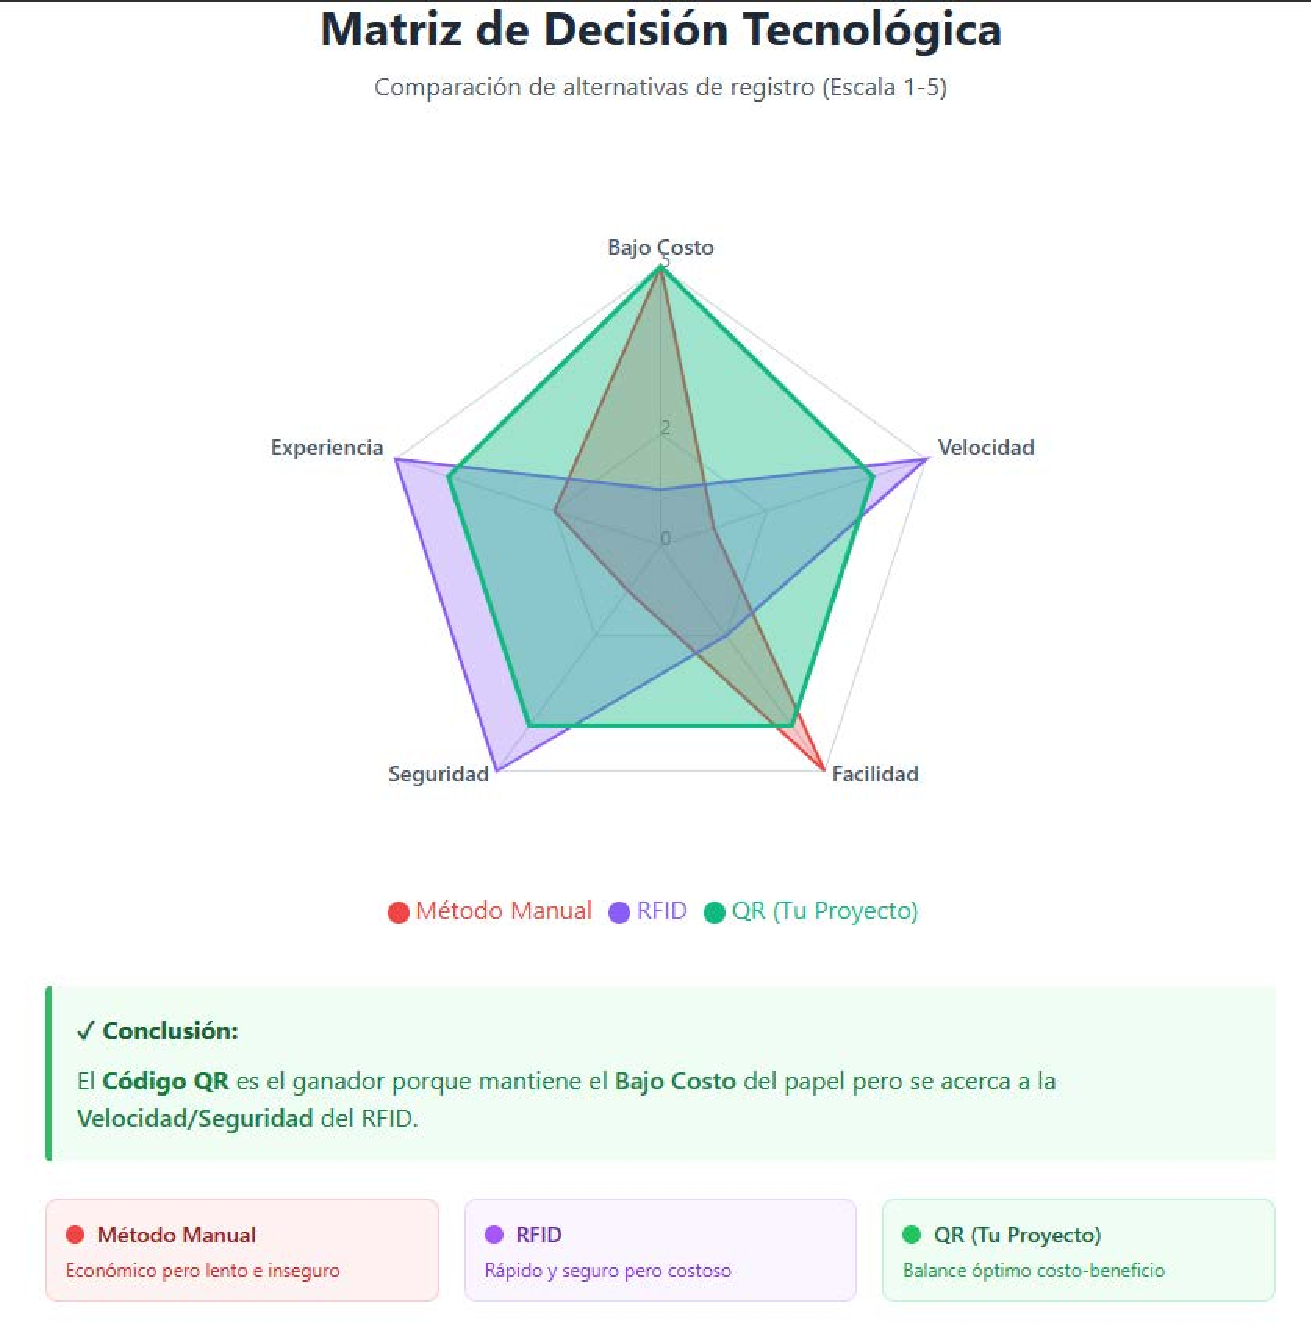
\includegraphics[width=0.45\textwidth]{graphics/Diagrama2.pdf}
    \caption{Comparación multi-criterio de tegnologias : RFID, Codigo QR y metodologia tradicional}
    \label{fig:comparacion_metodologias}
\end{figure}

Como resultado de este análisis, seleccionamos Scrum como metodología principal. Scrum mostró el mejor balance entre estructura suficiente para mantener al equipo organizado y flexibilidad para adaptarnos a cambios, factores que resultaron críticos en el contexto del proyecto. Trabajamos con sprints de dos semanas, lo que nos permitía entregar funcionalidades incrementales y recibir retroalimentación continua sin caer en el caos de cambios demasiado frecuentes.


\begin{table}[htbp]
\centering
\caption{Comparación de Tecnologías de Identificación para Asistencia}
\label{tab:frameworks}
\small
\renewcommand{\arraystretch}{0.8}
\begin{tabular}{lccc}
\toprule
\textbf{Tecnología} & \textbf{Costo} & \textbf{Velocidad} & \textbf{Seguridad} \\
\midrule
Método Tradicional (Papel) & Bajo & Lento & Baja \\
Código QR & Bajo & Rápido & Media \\
RFID & Alto & Muy Rápido & Alta \\
\bottomrule
\end{tabular}
\end{table}